\documentclass[class=NTHU_thesis, crop=false]{standalone}
\begin{document}

\chapter{Review on the MonoH Analysis}
\section{Dark Matter and the $Z^\prime$-2HDM Model}
In the universe, the galaxies are observed to violate Newton's second law with the rotation of the observable matters which is faster than expected. Thus it is thought that there are invisible matters called Dark Matter (DM) generating additional gravity to accelerate the rotation. The most popular hypothesis is proposed that DM is a stable and electrically natural particle $\chi$ which only has weak and gravitational interaction with the Standard Model (SM) particles. Thanks to the characteristics, we can try to search such particle at the Large Hadron Collider (LHC).

One possible model of DM is a Type-II two-Higgs-doublet model (2HDM) with an additional U(1)$_{Z^\prime}$ gauge symmetry, known as the $Z^\prime$-2HDM model. A light scalar $h$, which is identified as the SM Higgs boson, and a pseudo-scalar $A$ are introduced among this model, together with a striking process shown in Figure 3.1. The process has the attribute targeted by the collider searches that the final state is DM following with a detectable particle, the SM Higgs boson $h$ in this case. Due to the single visible Higgs boson in the final state, the search for DM of $Z^\prime$-2HDM model is called the monoH analysis. This analysis exploits the largest decay branching ratio of a Higgs boson into a pair of b-quarks. The following sections will briefly present the result of the analysis.

\fig[0.45][!hbt]{DM-Model.png}[The aimed process of the production of DM $\chi$ in the $Z^\prime$-2HDM model. A SM Higgs boson decaying to a pair of $b$ quarks is produced through a $Z^\prime$ mediator coupled to a pseudo-scalar Higgs boson $A$, which eventually decays to undetectable $\chi\bar{\chi}$.]

\section{Background Estimation Strategy}
The main background processes of the analysis are $Z$($\nu\nu$) + jets, $W$($l\nu$) + jets and $t\bar{t}$, shown in Figure 3.2. In the $Z$($\nu\nu$) + jets process, the undetectable neutrinos in the final state are regarded as the missing energy. Thus once the jets are tagged as $b$-jets, the case will be background. In the $W$($l\nu$) + jets process, once the lepton is misidentified as the missing energy and the jets are tagged as $b$-jets as mentioned previously, the procedure will be interference as well. In the $t\bar{t}$ case, if both the leptons are misidentified, the process will be background.

\begin{figure}[!hbt]
	\captionsetup[subfigure]{labelformat=empty}
	\centering
	\subcaptionbox
	{$Z$($\nu\nu$) + jets
		\label{fig:subfig_fig1}}
	{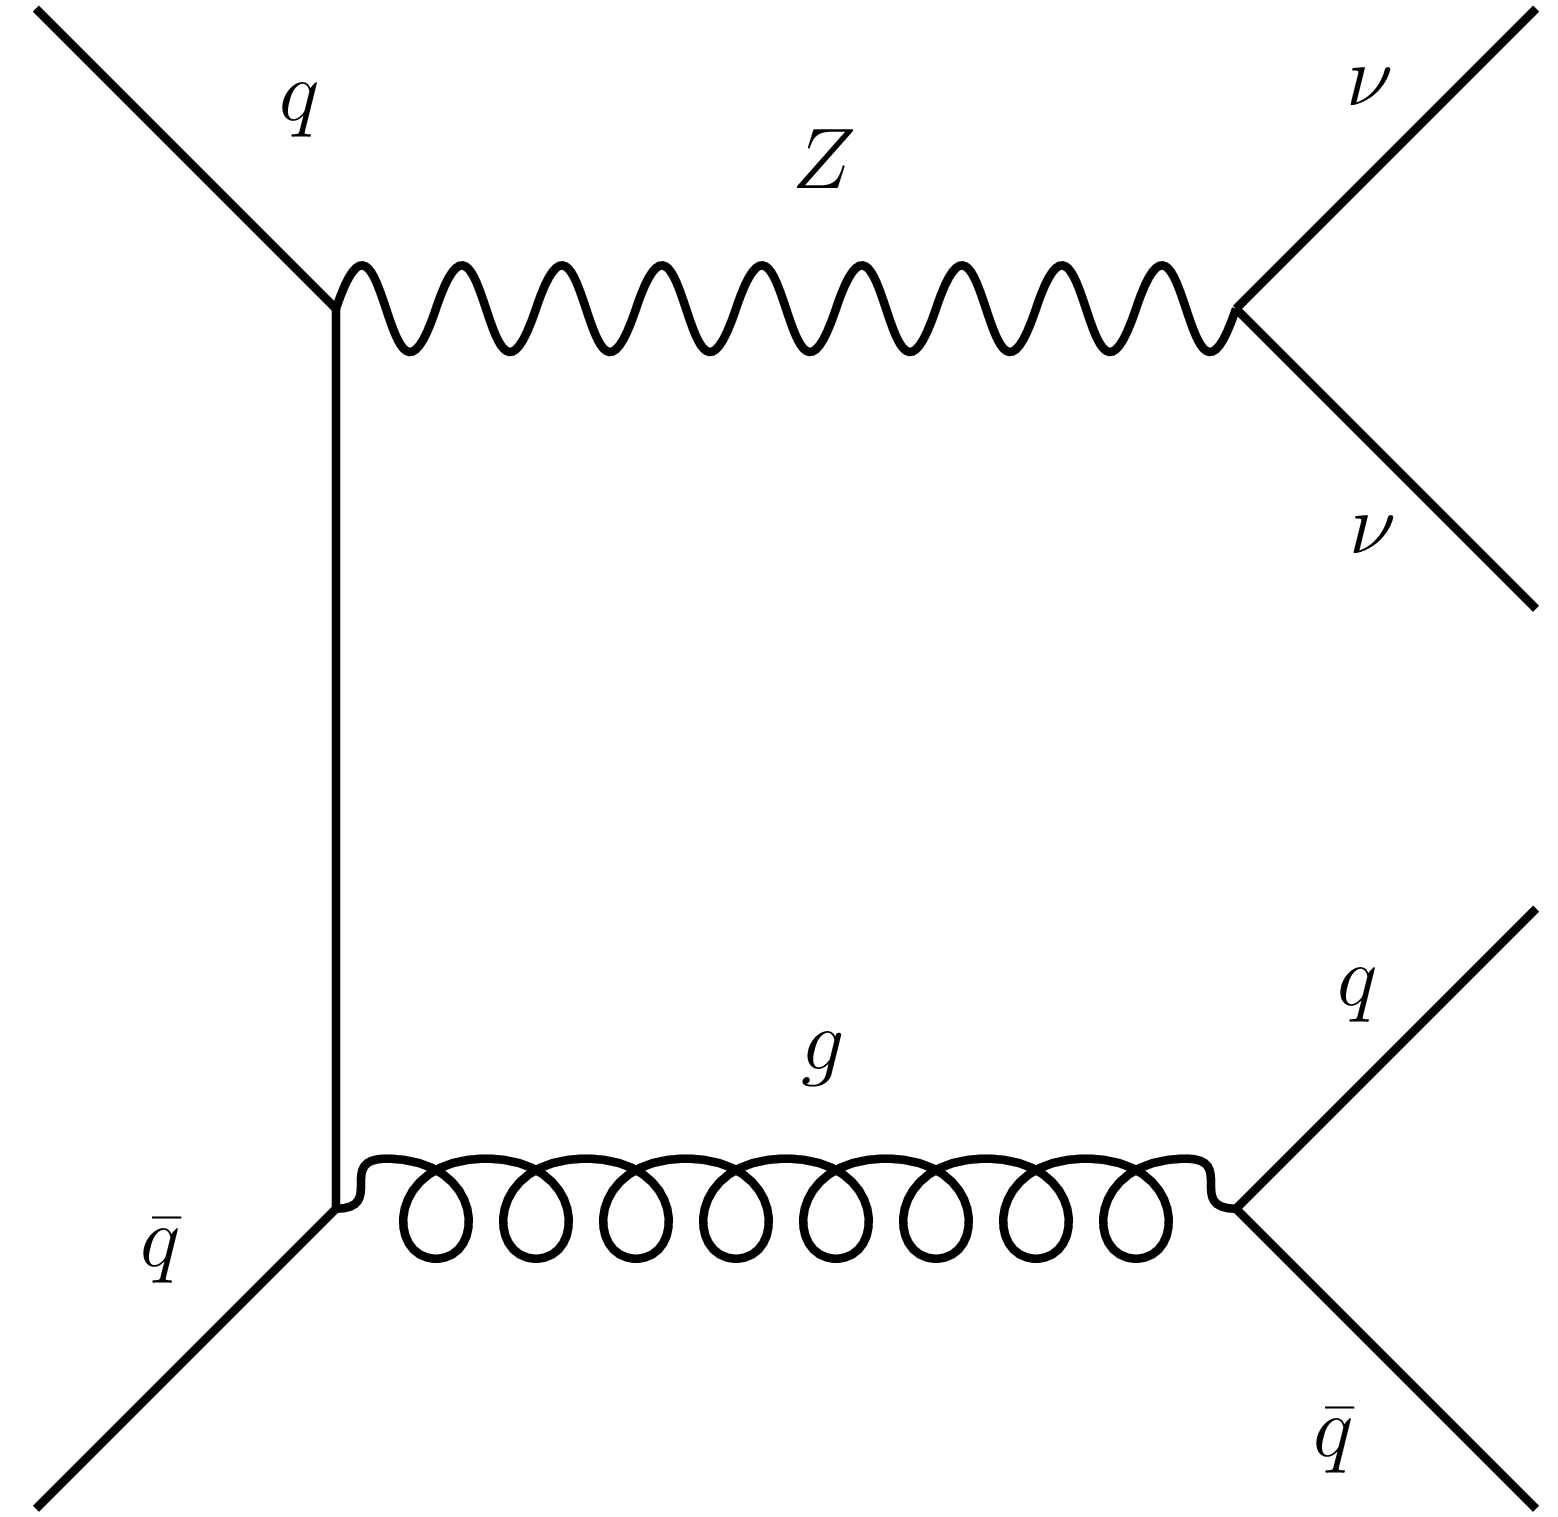
\includegraphics[width=0.3\linewidth]{Zvv.png}}
	~
	\subcaptionbox
	{$W$($l\nu$) + jets
		\label{fig:subfig_fig2}}
	{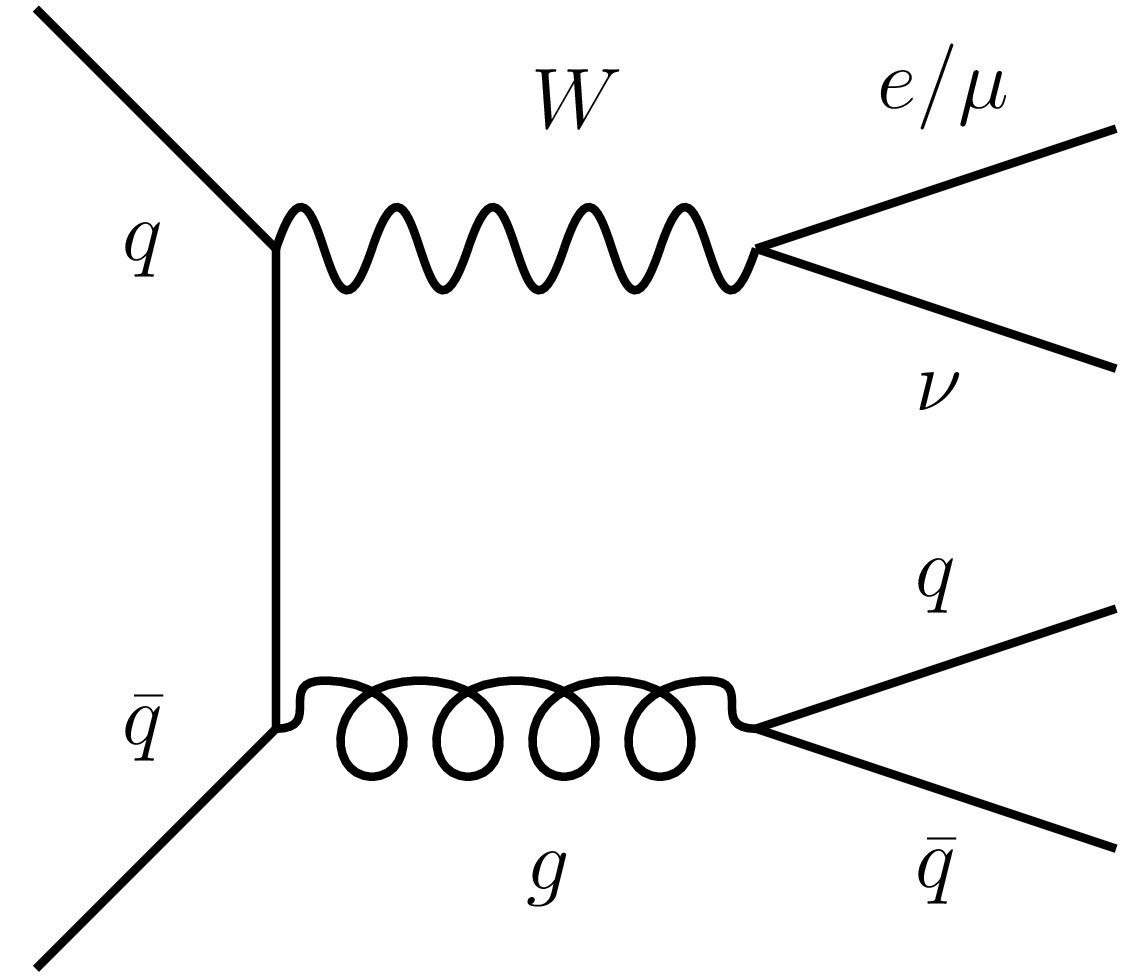
\includegraphics[width=0.3\linewidth]{Wlv.png}}
	~
	\subcaptionbox
	{$t\bar{t}$
		\label{fig:subfig_fig3}}
	{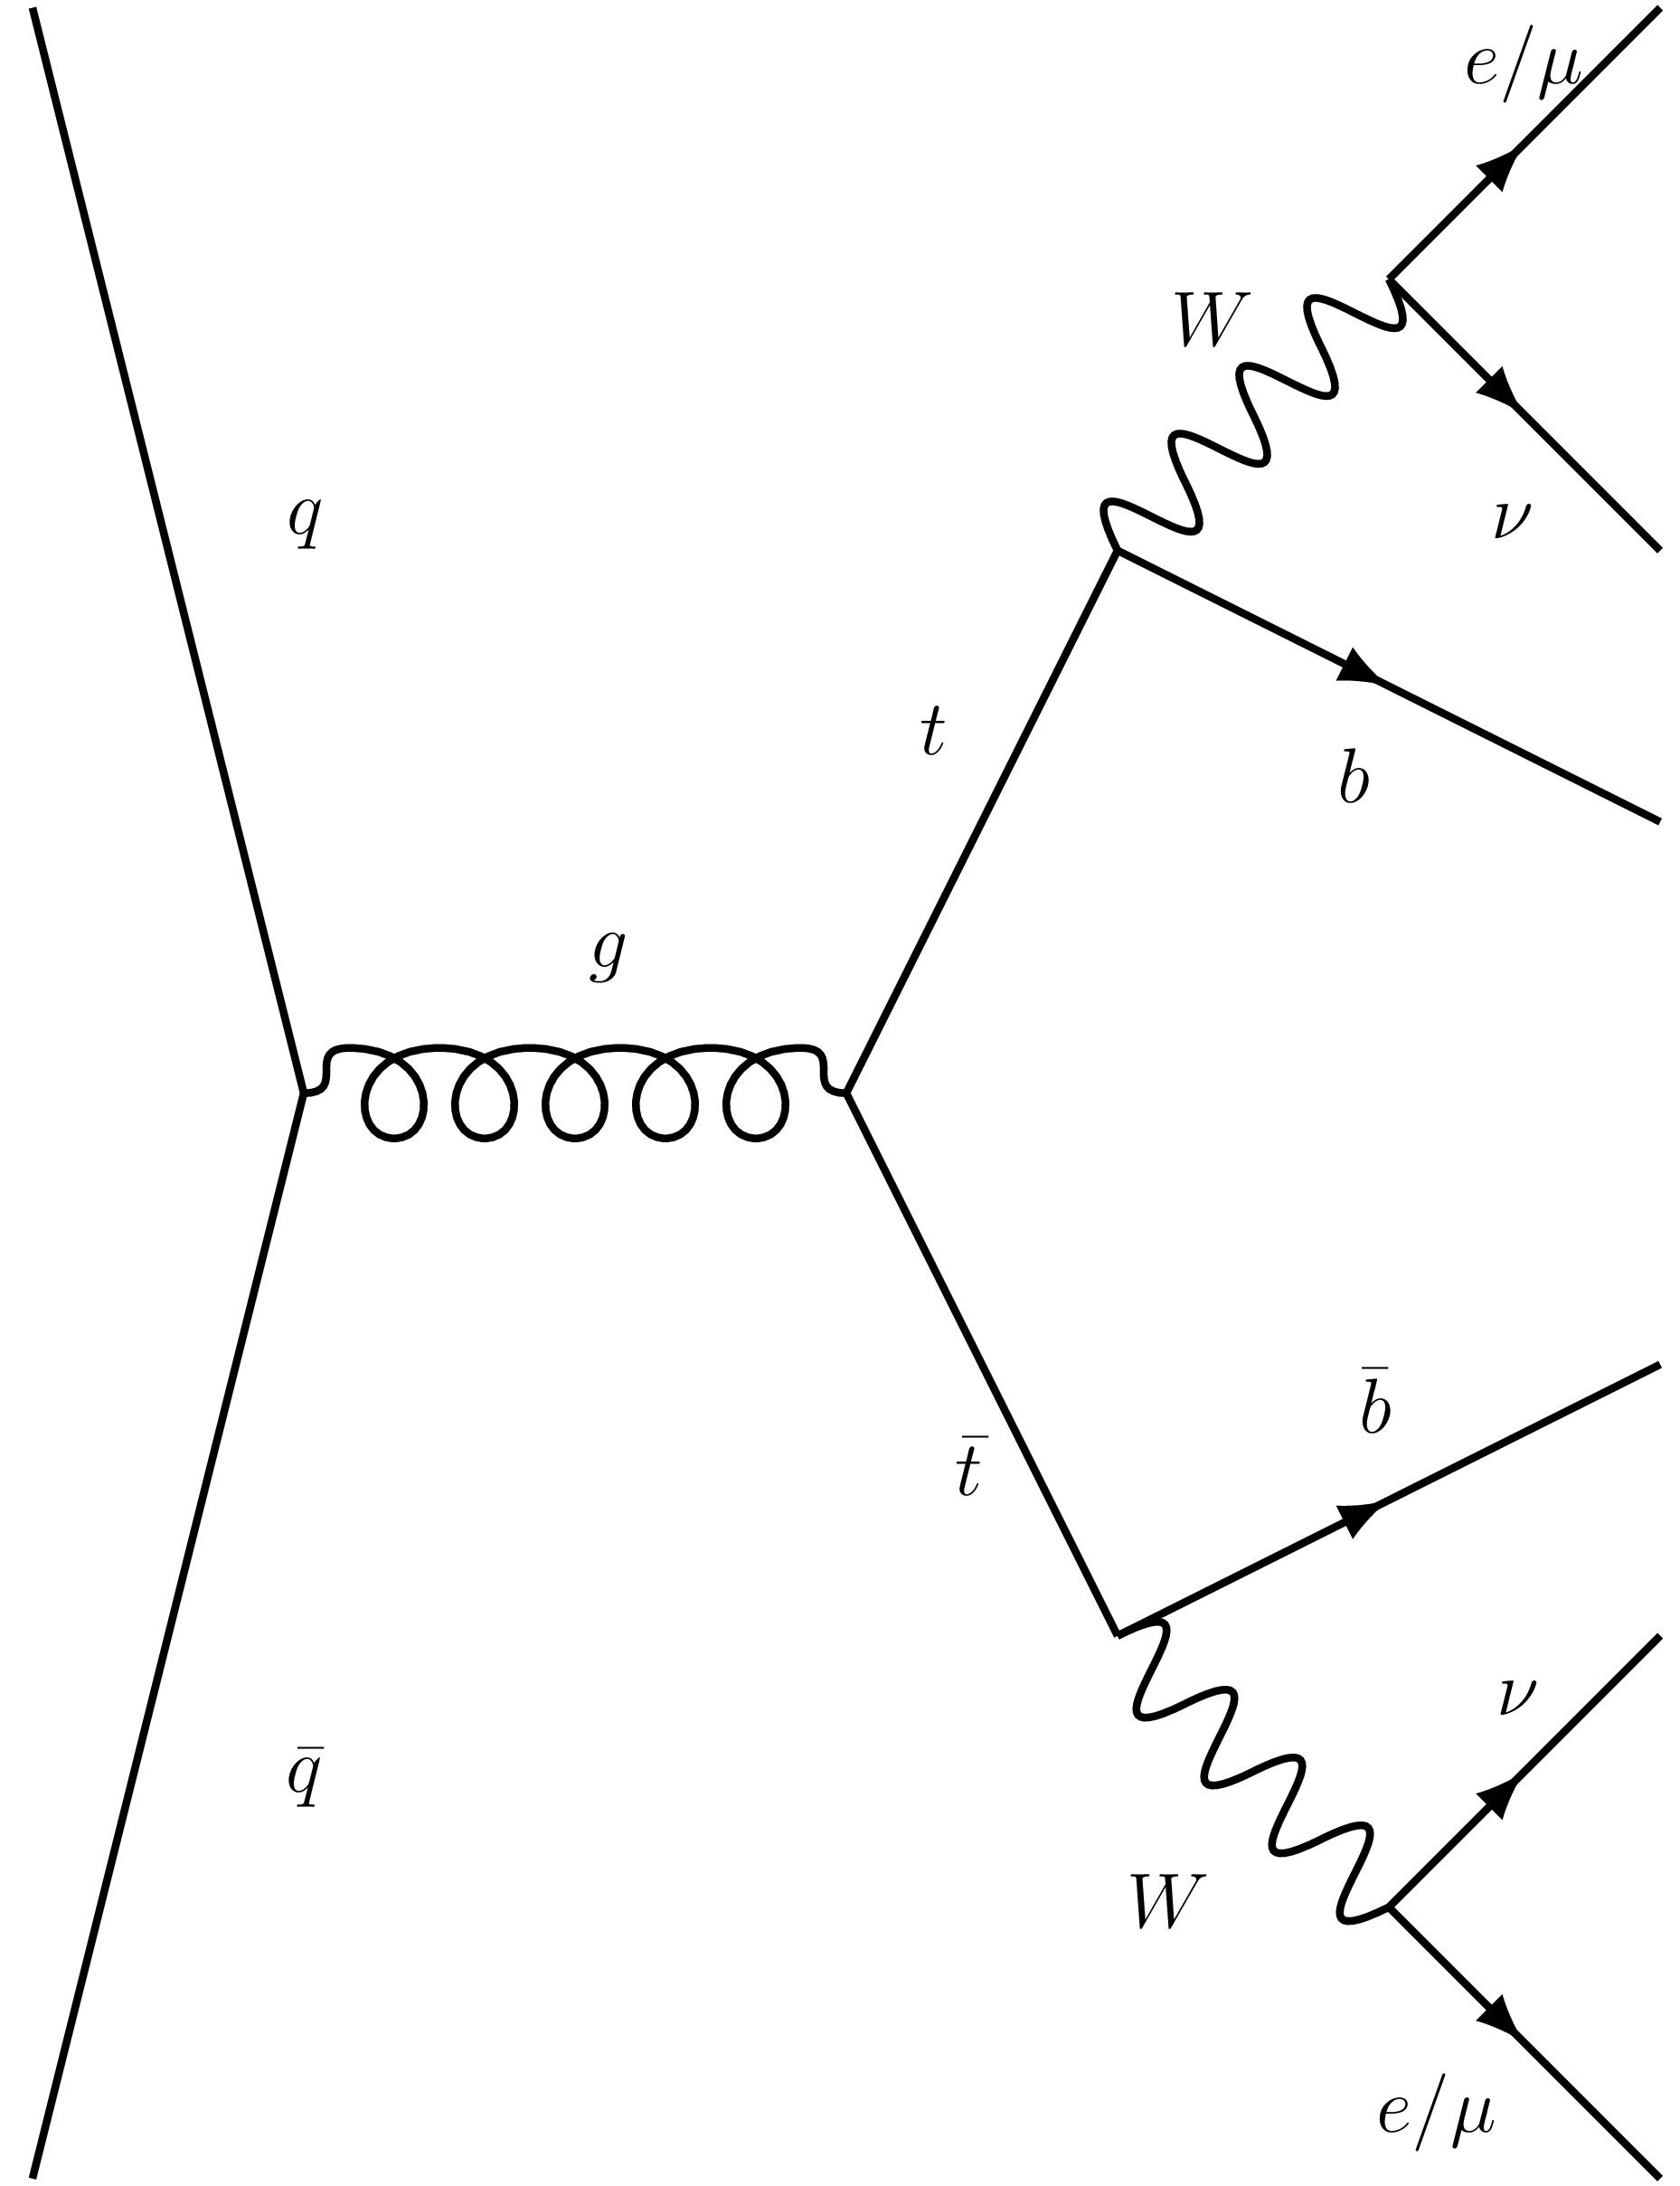
\includegraphics[width=0.3\linewidth]{ttbar.png}}
	\caption{The main background processes of the monoH analysis.}
	\label{fig:label}
\end{figure}

To constrain these background, the control region (CR) strategy is used. Before defining the CR, the signal region (SR) is defined as where the signals are expected to show. The SR is required to have no lepton based on the model. Then the CR is defined as the orthogonal region to the SR. Exploiting the similar kinematics, the CRs use some better-measured processes in order to constrain the background. There are two CRs in this analysis, the 1-lepton CR and the 2-lepton CR. The 1-lepton CR contains two processes, $W$($l\nu$) + jets and $t\bar{t}$, constraining the same processes in the SR. It requires different number of misidentified lepton, for $W$($l\nu$) + jets, one misidentified lepton in the SR but none in the 1-lepton CR, and for $t\bar{t}$, two misidentified leptons in the SR but one in the 1-lepton CR. The 2-lepton CR exploits the $Z$($ll$) + jets, constraining the $Z$($\nu\nu$) + jets process.

\section{Object Reconstruction and Selection}
\subsection{Jets}
Jets are a method to describe hadronic showers in detectors, consisting of multiple objects. Jets are reconstructed with the anti-$k_t$ algorithm. Depending on the toplogical clusters, the radius parameter of $R = 0.4$ is the small-radius (small-$R$) jets and of $R = 1.0$ is the large-radius (large-$R$) jets.

The small-$R$ jets with $p_T > 20 GeV$ for $\left|\eta\right| < 2.5$ are regarded to as the central jets. The MV2c10 discriminant is used for $b$-tagging the central jets to identify the $b$-hadrons, with the 77\% efficiency working point. In addition, the small-$R$ jets with $p_T > 30 GeV$ for $2.5 < \left|\eta\right| < 4.5$ are treated as the forward jets. The large-$R$ jets are required to have $p_T > 200 GeV$ and $\left|\eta\right| < 2.0$, containing multiple split jets called the track jets. The flavor identification for the large-$R$ jets depend on the ghost-associated track jets with the MV2c10 discriminant with the 77\% $b$-tagging efficiency working point. The track jets are depicted more in the following.

The fixed-radius (FR) track jets are applied for $b$-tagging in the previous analysis, using the anti-$k_t$ algorithm with fixed radius parameters. Instead of the FR track jets, the variable-radius (VR) track jets are implemented in the analysis for improving the $b$-tagging efficiency. The primary characteristic of the VR track jets is the relevance between the $p_T$ and the jet radius parameter: 
\begin{equation}
R \to R_{eff}(p_T) \approx \frac{\rho}{p_T}
\end{equation}
where $\rho$ is a constant factor. There are also two additional parameters, $R_{min}$ and $R_{max}$, as the radius boundary cut. The optimal values are respectively $\rho = 30 GeV$, $R_{min} = 0.02$ and $R_{max} = 0.4$.

\subsection{Leptons}
Electrons are reconstructed with energy deposits in the EM calorimeter which matches tracks in the ID. Besides the basic reconstruction, there are two types of electrons for the further selection in the analysis, the baseline electrons and the signal electrons. The baseline electrons have a loose criterion with $\left|\eta\right| < 2.47$ and $p_T < 7 GeV$, used for electron vetoes. For the events containing electrons, the signal electrons require $\left|\eta\right| < 2.47$ and $p_T < 27 GeV$.

The muon reconstruction relies on the muon spectrometer in the range of $\left|\eta\right| < 2.7$. It's also claimed to match the tracks in the ID for $\left|\eta\right| < 2.5$. Like electrons, there are two categories of muons, the baseline muons and the signal muons. The baseline muons are used for vetoing events in certain regions, requiring $\left|\eta\right| < 2.7$ and $p_T < 7 GeV$. The signal muons are defined with the criterion of $\left|\eta\right| < 2.5$ and $p_T < 25 GeV$ for the events which contain muons.

Because of the hadronic-like nature of taus, the reconstruction is complicated and described in Reference[]. For the tau vetoes in the analysis, the taus are required to have one or three tracks and have $\left|\eta\right| < 2.5$ and $p_T < 20 GeV$, excluding the crack region $1.37 < \left|\eta\right| < 1.52$.

\subsection{Missing Transverse Momentum}
The missing transverse momentum is determined as the negative vector sum of the transverse momentum of all the reconstructed and calibrated objects in an event. Additionally, the track-based soft term is added into the missing transverse momentum in the analysis, which is from the tracks that not associated with any reconstructed object but still linked to the primary vertex. The absolute value of the missing transverse momentum is expressed as $E^{miss}_T$, or MET. Also, there is a purely track-based missing transverse momentum calculated as the negative vector sum of the transverse momentum of all the reconstructed tracks associated with the primary vertex. The absolute value of the track-based missing transverse momentum is denoted as $p^{miss}_T$.

Furthermore, to recognize whether the MET is from weakly interacting particles or from the mismeasurement of multijet processes, two kinds of the MET significance are applied. One is the event-based MET significance which is performed in previous monoHbb analysis, and the other is the object-based MET significance which is newly introduced in the analysis. They will be depicted more detailed in the following section.

\section{Event Selection}
The SR is divided into two parts, the resolved region ($150 < E^{miss}_T < 500 GeV$) and the merged region ($E^{miss}_T > 500 GeV$), for different event selection requirements. As previously mentioned in 3.2, to be the comparison of the SR, the CRs are also divided into two divisions with the $p_T$ of the vector boson ($W$ or $Z$) as the separation boundary ($150 < p^V_T < 500 GeV$ for the resolved region and $p^V_T > 500 GeV$ for the merged region). The common selection among the SR and the CRs is introduced before the respective selection. The total event selection will be summarized in Table 1.

\subsection{Common Selection}


\subsection{Respective Selection}

MET sig

\section{Systematic Uncertainty}

\section{Results}
the improvement of this analysis
VR
object-based MET sig

\end{document}